\documentclass[12pt,a4paper]{report}

\usepackage[utf8]{inputenc} % pentru suport diacritice
\usepackage[romanian]{babel} % setări pentru limba română 
\renewcommand\familydefault{\sfdefault} % sans serif

\usepackage[margin=2.54cm]{geometry}	% dimensiuni pagină și margini
\usepackage{graphicx} % support the \includegraphics command and options

% formatting sections and subsections
\usepackage[section]{placeins}
\usepackage[ separate-uncertainty = true, multi-part-units = repeat]{siunitx}
\usepackage[nottoc,numbib]{tocbibind}
\usepackage{indentfirst}
\usepackage[parfill]{parskip}
\usepackage{textcase}
\usepackage[titletoc, title]{appendix}
\usepackage{titlesec}
\titleformat{\chapter}{\large\bfseries}{\thechapter}{2ex}{}[\vspace*{-1.5cm}]
\titleformat*{\section}{\large\bfseries}
\titleformat*{\subsection}{\large\bfseries}
\titleformat*{\subsubsection}{\large\bfseries}

\usepackage{chngcntr}
\counterwithout{figure}{chapter} % no chapter number in figure labels
\counterwithout{table}{chapter} % no chapter number in table labels
\counterwithout{equation}{chapter} % no chapter number in equation labels

\usepackage{booktabs} % for much better looking tables
\usepackage{url} % Useful for inserting web links nicely
\usepackage[bookmarks,unicode,hidelinks]{hyperref}

\usepackage{array} % for better arrays (eg matrices) in maths
\usepackage{paralist} % very flexible & customisable lists (eg. enumerate/itemize, etc.)
\usepackage{verbatim} % adds environment for commenting out blocks of text & for better verbatim
\usepackage{subfig} % make it possible to include more than one captioned figure/table in a single float
\usepackage{enumitem}
\setlist{noitemsep}

%%% HEADERS & FOOTERS
\usepackage{fancyhdr}
\pagestyle{empty}
\renewcommand{\headrulewidth}{0pt}
\renewcommand{\footrulewidth}{0pt}
\lhead{}\chead{}\rhead{}
\lfoot{}\cfoot{\thepage}\rfoot{}



\newcommand{\HeaderLineSpace}{-0.5cm}
\newcommand{\UniTextRO}{Universitatea POLITEHNICA București \\[\HeaderLineSpace] 
Facultatea Automatică și Calculatoare \\[\HeaderLineSpace]
Departamentul Automatică și Informatică Industrială\\}
\newcommand{\DiplomaRO}{LUCRARE DE LICENȚĂ}
\newcommand{\AdvisorRO}{Coordonator științific:}
\newcommand{\BucRO}{BUCUREȘTI}

\newcommand{\frontPage}[5]{
\begin{titlepage}
\begin{center}
{\Large #1}  % header (university, faculty, department)
\vspace{50pt}
\begin{tabular}{p{6cm}p{3cm}}

\includegraphics[scale=0.8]{pics/upb-logo.jpg} &
	
\includegraphics[scale=0.27,clip=true]{pics/acs_logo.jpg}
\end{tabular}

\vspace{105pt}
{\Huge #2}\\                           % diploma project text
\vspace{40pt}
{\Large #3}\\ \vspace{0pt}  % project title
\vspace{40pt}
{\LARGE \Name}\\                   % student name
\end{center}
\vspace{60pt}
\begin{tabular*}{\textwidth}{@{\extracolsep{\fill}}p{6cm}r}
&{\large\textbf{#4}}\vspace{10pt}\\      % scientific advisor
&{\large \Advisor}                                    % advisor name
\end{tabular*}
\vspace{20pt}
\begin{center}
{\large\textbf{#5}}\\                                % bucharest
\vspace{0pt}
{\normalsize \Year}
\end{center}
\end{titlepage}
}

\newcommand{\frontPageRO}{\frontPage{\UniTextRO}{\DiplomaRO}{\ProjectTitleRO}{\AdvisorRO}{\BucRO}}

\linespread{1.5}
\setlength\parindent{15pt}
\setlength\parskip{.28cm}

%% Abstract macro
\newcommand{\AbstractPage}{
\begin{titlepage}
\textbf{\large TODO:  SINOPSIS}\par
\AbstractRO\par\vfill
\end{titlepage}
}


%%%%%%%%%%%%%%%%%%%%%%%%%%%%%%%%%%%%%%%%%%%%%%%%%%   
%%
%%          End of template definitions
%%   
%%%%%%%%%%%%%%%%%%%%%%%%%%%%%%%%%%%%%%%%%%%%%%%%%%

\newcommand{\ProjectTitleRO}{Integrarea unei plăci de dezvoltare bazate pe microcontrolerul ATSAMR21 cu mediul de dezvoltare Arduino IDE}
\newcommand{\Name}{Blânzeanu Doru-Florin}
\newcommand{\Advisor}{SI. dr. ing. Radu Pietraru}
\newcommand{\Year}{2018}




% Setări document
\title{Proiect de diplomă}
\author{\Name}
\date{\Year}

\newcommand{\Thanks}{(opțional) Aici puteți introduce o secțiunea specială de mulțumiri / acknowledgments. }

\newcommand{\AbstractRO}{Sinopsisul proiectului are rol de introducere, conținând atât o descriere pe scurt a problemei abordate cât și o enumerare sumară a rezultatelor și a concluziilor. Se recomandă ca sinopsisul să fie redactat într-un limbaj accesibil unei persoane nefamiliarizate cu domeniul, dar în același timp destul de specific pentru a oferi rapid o vedere de ansamblu asupra proiectului prezentat.
Sinopsisul proiectului va fi redactat atât în română cât și în engleză. Ca dimensiunea recomandată aceasta secțiune va avea maxim 200 de cuvinte pentru fiecare variantă. Împreună, ambele variante se vor încadra într-o singură pagină.}

\begin{document}

\frontPageRO

%empty page
\clearpage
\thispagestyle{empty}
\phantom{a}
\vfill
\newpage
\vfill

\begingroup
\linespread{1}
\tableofcontents
\endgroup

%empty page
\clearpage
\thispagestyle{empty}
\phantom{a}
\vfill
\newpage
\vfill

\chapter{Introducere}\pagestyle{fancy}
În lucrarea de față se va vorbi despre integrarea unei noi plăci de dezvoltare, Atmel SAMR21 Xplained Pro, în ecosistemul Arduino. Deasemenea, se va face o analiză asupra domeniului Internetului Lucrurilor(IoT)\footnote{IoT = Internetul of Things} în care se utilizează microcontrolerul acestei placi de dezvoltare și a importanței circuitelor care îmbină puterea de calcul cu comunicația radio.

Pentru dezvoltarea de sisteme integrate exista opțiunea de a alege componenta de bază pentru procesare fie un microcontroler, fie un microprocesor. Ambele abordări au avantajele și dezavantajele lor, dar în general în aplicațiile în care contează dimensiunea, costul și puterea consumată, este preferat un microcontroler. Când vine vorba despre o aplicație care necesită comunicație radio, alegerea unui microcontroler care are integrată o componentă radio este mult mai convenabilă spre deosebire de un microcontroler care nu dispune de această componentă la care să se adauge componenta radio externă. Unul dintre motivele pentru care este mai convenabilă prima variantă este constrângerea asupra dimensiunii, care în cazul primei opțiuni, este mult mai mică.
Un alt motiv pentru care reprezintă un avantaj prima opțiune este faptul că producătorii acestor microcontrolere au ca scop maximizarea performanței prin minimizarea consumului, astfel aceste microcontrolere sunt specializate în comunicația radio spre deosebire de celelalte care sunt de uz general.


Arduino este o platformă open-source bazată pe componente hardware și unelte software ușor de utilizat. Ecosistemul Arduino oferă suport și pentru o gamă largă de alte microcontrolere, toate aceste unelte alăturate într-un singur pachet ușor de utilizat pentru dezvoltatorii începători, însă destul de flexibil pentru dezvoltatorii avansați.
Arduino este foarte utilizat in diverse domenii cum ar fi:
\begin{itemize}
	\item robotică
	\item internetul lucrurilor
	\item învățământ
	\item prototipare
	\item cercetare și dezvoltare
\end{itemize}

Datorită faptului că Arduino este o platformă open-source, oricine este binevenit să contribuie la dezvoltarea de noi funcționalități și integrarea de noi plăci de dezvoltare. Acest lucru are și avantajul că exisă mulți utilizatori care lucrează pe același cod sursă, astfel totodată involuntar testând și raportând orice tip de problemă.

În ultimii ani, Arduino a atras din ce în ce mai mulți utilizatori dornici să implementeze aplicații practice rapid deoarece arhitectura platformei are grijă să inițializeze și să configureze multe dintre elementele utilizate, astfel este mult mai simplu pentru utilizatorii mai puțin experimentați să înceapă un proiect nou, iar utilizatorii cu experiență pot opta să configureze manual doar elementele sau modulele de care ei au nevoie. 


\chapter{Prezentarea domeniului din care face parte lucrarea}
Internetul Lucrurilor se referă la un tip de rețea care conectează totul la internet printr-o suită de protocoale în scopul schimbării de  informație și a comunicării pentru a putea implementa recunoaștere, poziționare, urmărire și administrare inteligentă\cite{theiot}. \\
Internetul lucrurilor promite să revoluționeze felul în care noi trăim și muncim. Ne-ar putea ajuta să trecem peste problemele globale datorate populației: criza energiei, lipsa resurselor și poluare. Pentru a realiza această viziune, avem nevoie de senzori care preiau informația din mediu și o împărtășesc între ei sau cu alte dispozitive care permit accesul utilizatorului uman pentru a lua decizii inteligente care afecteaza întregul nostru ecosistem.
Datorită acestui fapt, interesul către internetul lucrurilor este din ce în ce mai mare. Multe studii au prevăzut o creștere accelerată a numărului de vânzări de dispozitive inteligente în următorii 10 ani.

Imaginați-vă o lume în care milioane de obiecte, dispozitive are putea comunica și împărtăși informația între ele, toate interconectate printr-o rețea internet. Toate datele colectate de acele obiecte(senzori) fiind centralizate în anumite centre de colectare a datelor care au o interfață de expunere către utilizator. \\
Aplicațiile care se pot dezvolta ulterior să folosească acele date pot ajuta omenirea în diverse domenii: industrie, sănătate, stil de viață, comunicații, etc.
Ne apropiem cu pași repezi de acel ideal, însă suntem deocamdată departe deoarece există încă destule probleme care apar din cauza multor factori precum:
\begin{itemize}
	\item cost
	\item securitate
	\item performanță
	\item consum
\end{itemize}

Potrivit unui studiu efectuat în anul 2018 cu privire la clasificarea domeniilor în care activează proiecte din domeniul internetului lucrurilor spune că majoritatea proiectelor sunt în sectorul de orașe inteligente, industrie și clădiri inteligente\cite{study}. Pe continentul american se află majoritatea acestor proiecte, urmat de Europa și Asia. Există diferențe mari între regiuni și domeniile de activitate ale proiectelor, astfel majoritatea proiectelor pentru orașe inteligente se află pe teritoriul european în timp ce pe continentul american predomină proiecte de mașini inteligente și sănătate. Asia este puternic dezvoltată în domeniul agriculturii inteligente.

Dorința de a funcționa un timp îndelungat fără să necesite intervenția omului, a fost scopul principal în designul de rețele de senzori wireless în ultimii 10 ani\cite{lowpowervsperformance}. Prin concentrarea asupra acestei cerințe, designerii au căutat acele componente hardware care aveau cel mai mic consum de curent electric în mod activ și în sleep mode\footnote{sleep mode = mod de consum redus}. Aceste dispozitive consumă energie de ordin mW putere în mod activ, iar în modul de consum redus uW, renunțând la putere de calcul și memorie în favoarea consumului redus.
În schimb, puterea de calcul limitată și resursele de memorie mici ale acestor platforme restricționează aplicațiile pe care le pot implementa. Aplicațiile tipice urmăresc un model care preia date de la senzori, îi stochează, îi trimite și apoi intră din nou în modul de consum redus, în care senzorii de pe placă sunt interogați și datele returnate sunt trimise către un server. Aplicațiile ce necesită putere de calcul mare nu sunt suportate de aceste platforme. \\
Aplicațiile care necesită putere de calcul mare sau procesare de semnal, în general trebuie să facă un compromis pentru a evita limitările impuse de platformă. Aceste aplicații tind să fie caracterizate de intervale alternante de activitate intensă urmată de perioade de inactivitate. Alternativa este să se utilizeze platforme care sacrifică consumul în favoarea puterii de procesare, sau platforme care combină microcontrolere low-power\footnote{low-power = consum redus} cu procesoare de înaltă performanță care consumă mult.

\section{Aplicații}
Internetul lucrurilor se poate aplica în activitățile industriale, inclusiv în tranzacțiile dintre companii, organizații sau alte entități, se poate utiliza în logistică, producție, procese, servicii, banking, etc\cite{iotfields}.
\subsection{Industrie}

\subsubsection{Logistică și managementul ciclului de viață al produsului}
În logistică și managementul ciclului de viață al produsului un exemplu bun de utilizare a internetului lucrurilor este în procesul de selecție a produselor. Există etichete electronice atașate pe anumite obiecte care pot fi utilizate în identificarea tipului de material: îmbrăcăminte, mobilier, echipamente, alimente sau băuturi. Utilizarea etichetelor electronice contribuie la gestionarea eficientă a spațiului de depozitare și reduce inventarul. Întregul proces poate fi urmărit, spre exemplu utilizând un cititor de carduri RFID\footnote{RFID = Radio-frequency identification} instalat la o fabrică care poate monitoriza procesul de producție și fiecărei etichete i se poate vedea întreg parcursul în fabrică. Un sistem avansat compus din echipament RFID și urmărire în timp real a produselor de pe rafturi poate ajuta în reducerea deșeurilor, astfel reducând din costuri.

\subsubsection{Agricultură și creșterea animalelor}
În acest domeniu, internetul lucrurilor, contribuie prin urmărirea în timp real a poziției animalelor pentru a putea raporta în caz de anumite evenimente, cum ar fi boli, către autorități în timp util. Sistemele IoT de identificare permit monitorizarea și identificarea animalelor și izolează animalele infectate de animalele sănătoase, astfel evitând răspândirea bolilor infecțioase. Există sisteme avansate care pot memora informații despre condițiile fizice ale animalelor și le pot transmite astfel facilitând analiza datelor colectate pe care autoritățile le pot verifica.\\
Un alt exemplu bun din agricultură sunt fermele inteligente care au devenit visul oricărui fermier, să poți supraveghea cultura, să poți acționa de la distanță în consecință și să poți monitoriza starea solului în timp real sunt doar câteva dintre aplicațiile pe care le oferă IoT.

\subsubsection{Procese industriale}
În industria automobilelor, domeniul IoT are o vastă aplicabilitate, de la senzori de monitorizare a parametrilor funcționării automobilului, presiune în pneuri, consum de carburant, poziție, distanțe față de alte vehicule, până la automatizarea proceselor din industrie și a liniilor de fabricație. Datele de la senzorii amplasați în sistem pot oferi detalii importante care ușurează identificarea problemelor și rezolvarea acestora. 

\subsection{Oraș inteligent}
IoT va îmbunătăți susținerea mediului și calitatea vieții oamenilor. Principala resursă este energia și modul eficient de utilizare al acesteia, precum și soluții inteligente pentru îmbunătățirea vieții de zi cu zi a oamenilor.

\subsubsection{Clădiri inteligente}
Integrarea tehnologiei de comunicație în clădiri inteligente permite ca viitoarele clădiri sau orașe inteligente să fie echipate cu o varietate de senzori și dispozitive inteligente inter-conectate precum:
\begin{itemize}
	\item{telefoane mobile}
	\item{computer}
	\item{TV}
	\item{camere de supraveghere}
	\item{electrocasnice inteligente}
\end{itemize}
Unele aplicații permit funcții de bază IoT cum ar fi: sisteme de supraveghere, sistem de gestionare și mentenanță a fabricilor, sisteme multimedia; în timp ce alte aplicații integrează smart grid\footnote{smart grid = electrical grid which includes a variety of operational and energy measures} și optimizează consumul energiei. Spre exemplu, HAN\footnote{HAN = Home Area Network} permite electrocasnicelor să interacționeze cu instrumente inteligente, și asigură performanța cerută reducând costul. Poate deasemnea să programeze aceste electrocasnice să nu funcționeze în perioada de vârf. Toate aceste informații sunt accesibile utilizatorilor prin intermediul unei aplicații mobile.
\begin{figure}[th]
\centering
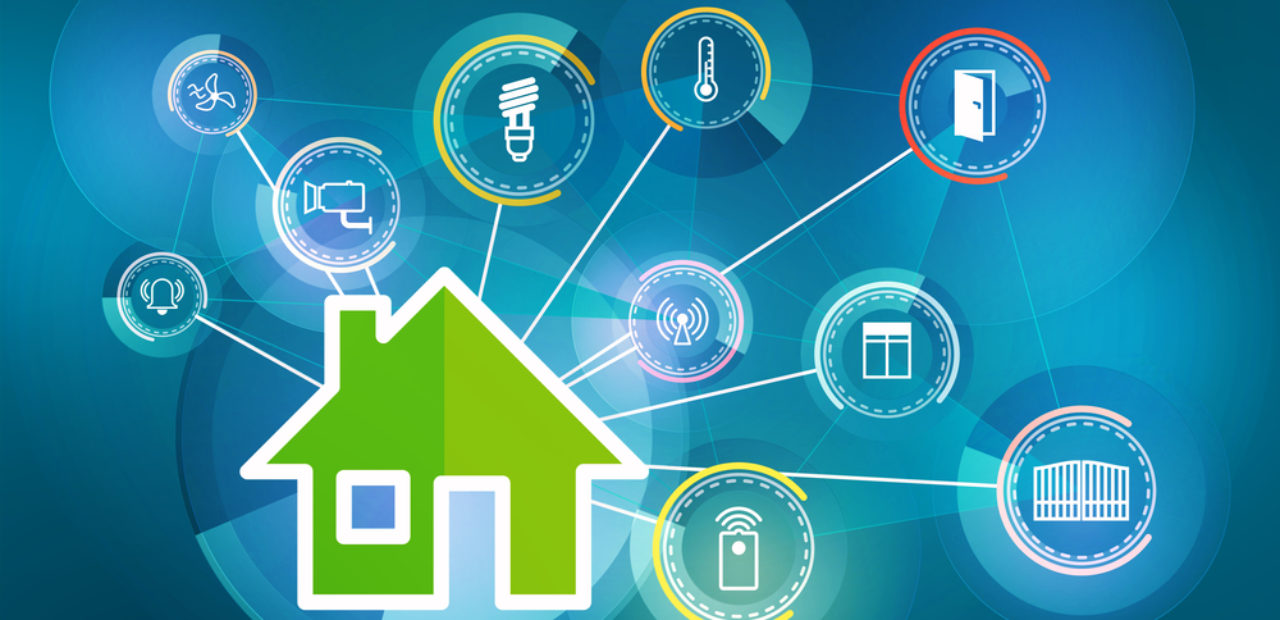
\includegraphics{pics/iot_home.jpg}
  \caption{Interconectarea sistemelor inteligente din clădiri}
  \label{fig:iot_home}
\end{figure}

\subsubsection{Siguranță publică și monitorizarea mediului}
Siguranța publică include menținerea ordinii publice, protecția cetățenilor și protecția de proprietate publică și privată. IoT oferă soluții de monitorizare și urmărire a situațiilor de urgență. Sistemele de urgență ajută la prevenirea și răspunsul în consecință în cazul unui cataclism. Prin colecționarea datelor de la camerele de luat vederi publice sau private se poate ajuta poliția să păstreze liniștea publică. Clădirile care necesită o securitate mai ridicată pot beneficia de sisteme IoT pentru protecție și detecție împotriva intrușilor. Senzori dedicați și camere inteligente,  sistemul GPS\footnote{GPS = Global Positioning System} care oferă date despre poziționare, locație în timp real, precum și utilizarea tehnologiei wireless\footnote{wireless = fără fir} pot ajuta la anticiparea anumitor evenimente.

\subsection{Sănătate}
Internetul lucrurilor va juca un rol important în dezvoltarea de servicii inteligente pentru îmbunătățirea activității sociale a oamenilor. IoT care implică cetățeni și comunități în guvernare și luare de decizii pentru a permite oamenilor să trăiască independent sau să mențină relații sociale și să îmbunătățească sănătatea.

\subsubsection{Diagnosticarea bolilor și tratament}
Industria sănătății va fi puternic influențată de IoT. Senzori inteligenți care permit colectarea de informații vitale de la pacienți(temperatură, tensiune arterială, puls, nivel de colesterol) în timp real  și transmise către un specialist printr-o tehnică de comunicație pentru diagnostic și monitorizare. Rețele BAN\footnote{BAN = Body Area Network} sunt interconectate prin dispozitive purtabile care permit monitorizare de la distanță a pacienților din afara spitalelor. Deasemenea IoT mai poate fi utilizat în identificarea substanțelor, ustensilelor în spitale și inventarierea acestora, astfel pierderea sau furtul acestora fiind mai puțin probabile.

\subsubsection{Stil de viață}
În cadrul acestui subdomeniu, IoT are o largă întrebuințare. Oamenii pot opta să utilizeze dispozitive purtabile care includ senzori de monitorizare a semnelor vitale care pot declanșa alarme medicale în cazul unor probleme de sănătate, precum și ale altor indici de interes pentru utilizator(calorii consumate, distanță parcursă, poziționare). Activitățile zilnice pot fi și acestea urmărite și se pot primi sugestii de schimbare a unor obiceiuri în funcție de scopul setat de utilizator. Pentru persoanele cu handicap vizual sunt dezvoltate aplicații IoT(senzori și aplicații mobile) care le ajută pe acestea să se deplaseze în oraș. 
\begin{figure}[th]
\centering
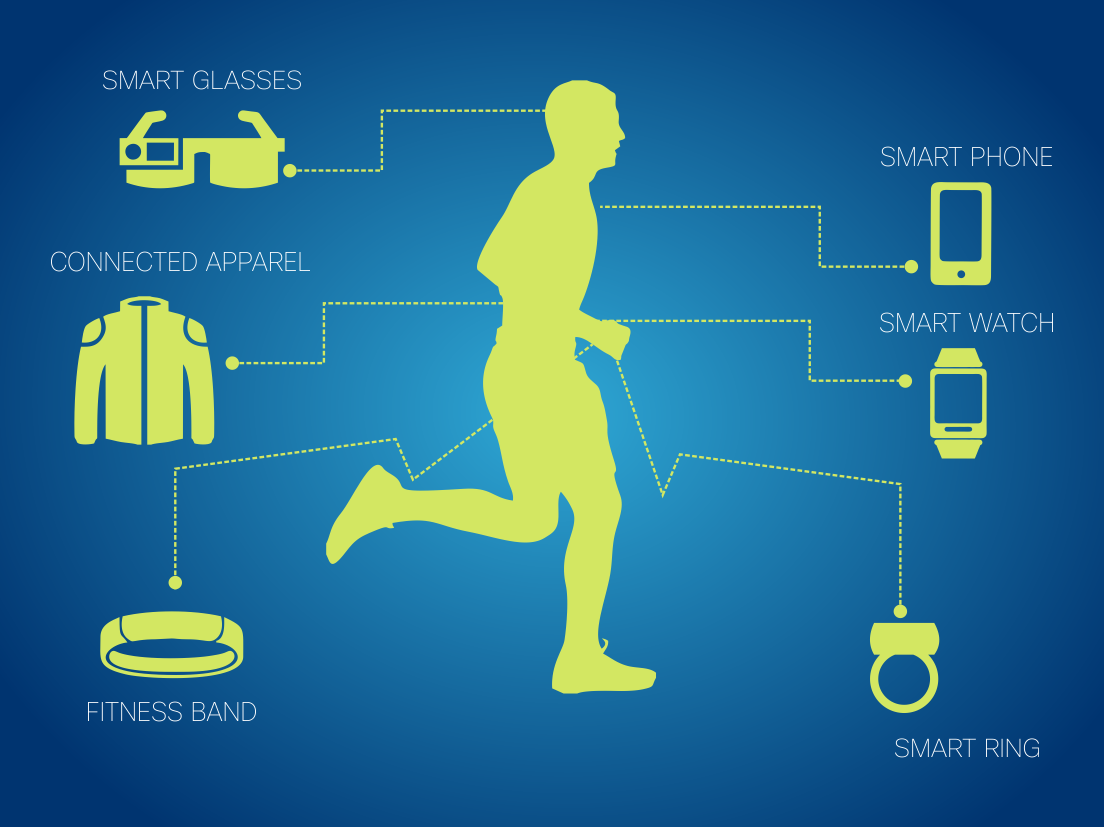
\includegraphics{pics/iot_health.png}
  \caption{Exemplu de sisteme ce ajută la îmbunătățirea stilului de viață}
  \label{fig:iot_health}
\end{figure}

\chapter{Descrierea problemei abordate și a metodei de rezolvare propuse}
În cadrul lucrării se abordează problematica integrării unei noi plăci de dezvoltare în ecosistemul Arduino. \\
Gama SAMR21 de la Atmel cuprinde o serie de microcontrolere cu consum redus ce pot fi utilizate în aplicații care necesită comunicație radio. Kitul de dezvoltare Atmel SAM R21 Xplained Pro este o platformă hardware proiectată de Atmel pentru a se putea evalua microcontrolerul ATSAMR21G18A. \\
Motivele pentru care un dezvoltator de aplicații IoT ar alege o placă de dezvoltare bazată pe microcontrolerul ATSAMR21G18A sunt:
\begin{itemize}
	\item{consumul redus}
	\item{performanța ridicată}
	\item{modulul radio integrat}
\end{itemize}
Când vine vorba de alegerea unui mediu de dezvoltare prietenos cu utilizatorii începători și care suportă o gamă largă de platforme și plăci de dezvoltare, opțiunile sunt limitate, cea mai des aleasă  metodă este utilizarea Arduino IDE. 
Arduino IDE permite utilizatorilor să dezvolte aplicații care folosesc plăci de dezvoltare bazate pe microcontrolere: AVR, SAMD, STM32, Intel ix86, etc. După cum se observă, plăcile de dezvoltare bazate pe microcontrolere SAMR, nu sunt suportate. \\
Tema propusă este să se adauge, la lista de plăci de dezvoltare suportate de către Arduino IDE, și placa Atmel SAMR21 Xplained Pro.

Primul pas în rezolvarea acestei probleme este de a analiza structura proiectului unei alte plăci de dezvoltare și a urma acel model. După analiza proiectului unei plăci de dezvoltare bazate pe SAMD s-a ajuns la concluzia că pentru adăuga o placă de dezvoltare la Arduino IDE trebuie să adăugăm o nouă componentă nucleu care să fie compatibilă cu placa de dezvoltare Atmel SAMR21 Xplained Pro și fișiere de configurare pentru pinii plăcii. 

\chapter{Documentație tehnică}
În capitolul curent se vor prezenta detaliile tehnice folosite în rezolvarea temei propuse.\\
\section{Placa Atmel SAMR21 Xplained Pro}
Pentru a putea duce la bun sfârșit tema propusă, au fost necesare două plăci de dezvoltare bazate pe microcontrolerul ATSAMR21G18A, două plăci Atmel SAM R21 Xplained Pro (Figura ~\ref{fig:samr21}). \\
Placa de dezvoltare Atmel SAM R21 Xplained Pro este o platformă hardware de evaluare a microcontrolerului ATSAMR21G18A, produs de Atmel\cite{samr21ug}. \\
\begin{figure}[th]
\centering
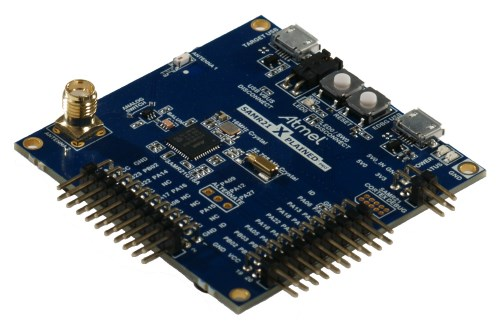
\includegraphics[scale=0.7]{pics/samr21.jpg}
  \caption{Atmel SAMR21 Xplained Pro}
  \label{fig:samr21}
\end{figure}\\
Cele mai importante caracteristici ale plăcii de dezvoltare sunt:
\begin{itemize}
	\item{procesor ARM Cortex-M0+ de până la 48MHz}
	\item{memorie flash 256KB}
	\item{memorie SRAM 32KB}
	\item{mod de consum redus}
	\item{depanator integrat(EDBG)}
		\subitem{interfață USB\footnote{USB = Universal Serial Bus}}
		\subitem{programarea și depanarea prin SWD\footnote{SWD = Serial Wire Debug}}
	\item{pini de intrare și ieșire}
	\item{două butoane mecanice}
	\item{un LED}
	\item{antenă radio}
		\subitem{antenă ceramică\cite{antena}}
		\subitem{un conector SMA\footnote{SMA = SubMiniature version A} pentru antenă externă}
	\item{trei posibilități de alimentare}
		\subitem{extern}
		\subitem{prin depanator USB}
		\subitem{prin USB țintă}
	\item{modulu radio AT86RF233\cite{at86rf}}
	\item{cristal de 32kHz}
	\item{cristal de 16MHz}
\end{itemize}

\subsection{Procesor}
Procesorul ARM Cortex-M0 + operează pe cuvinte de 32 de biți și a fost proiectat cu scopul de a servi în aplicații cu sisteme integrate\cite{cpu}. Oferă beneficii semnificative dezvoltatorilor, inclusiv:
\begin{itemize}
	\item{arhitectură simplu de învățat și utilizat}
	\item{mod de consum ultra redus}
	\item{procesare de întreruperi de mare performanță}
	\item{compatibil cu procesoare Cortex-M}
	\item{include sistem de protecție a memoriei}
\end{itemize}
Procesorul Cortex-M0+ este construit pe un nucleu optimizat pentru consum și dimensiune, cu un pipeline pe două niveluri și o arhitectură von Neumann.
Acest procesor implementează arhitectura ARMv6-M, care e bazată pe un set de instrucțiuni de 16 biți Thumb și include tehnologie Thumb-2. Acest lucru oferă performanțele excepționale așteptate de la un procesor cu arhitectură pe 32 de biți, cu o densitate mai mare a codului decât microcontrolerele de 8 sau 16 biți.

\subsection{Depanatorul integrat}
Placa Atmel SAM R21 Xplained Pro conține depanatorul Atmel EDBG\footnote{EDBG = Atmel Embedded Debugger} pentru depanarea codului sursă direct pe placa de dezvoltare. EDBG este compus din trei interfețe: un depanator, un port de comunicație serială COM\footnote{COM = Communication Port} și o interfață de date DGI\footnote{DGI = Data Gateway Interface}.\\
Depanatorul este utilizat pentru depanarea codului prin rularea lui pe placa de dezvoltare și verificarea bunei funcționări.\\
Portul de comunicație serială este conectat la o interfață UART\footnote{UART = Universal Asynchronous receiver-transmitter}, interfață de comunicație serială asincronă, și oferă posibilitatea de comunicare cu microcontrolerul prin terminal software. Oferă viteză de transfer ridicată, opțiuni de paritate a datelor transmise și de bit de stop.\\
Interfața de date e compusă din mai multe interfețe de comunicație cu computerul gazdă. Comunicația pe aceste interfețe este bidirecțională și poate fi folosită pentru notificarea în legătură cu declanșarea unor evenimente sau pur și simplu pentru transmisie de date.

\subsection{Surse de alimentare}
Placa de dezvoltare Atmel SAM R21 Xplained Pro poate fi alimentată în mai multe moduri, după cum arată tabela ~\ref{tab:surse}. \\
Placa de dezvoltare va detecta automat ce surse de alimentare sunt disponibile și va alege dintre acestea în funcție de următoarele priorități:
\begin{enumerate}
	\item{Extern}
	\item{Prin depanator USB}
	\item{Prin USB țintă}
\end{enumerate}

\begin{table}[th]\small\linespread{1}
\caption{Surse alimentare}
\label{tab:surse}
\begin{tabular}{l >{\raggedright\arraybackslash}p{8cm} >{\raggedright\arraybackslash}p{4cm}}
\textbf{Intrare} & \textbf{Tensiune} & \textbf{Curent} \\\hline
\textbf{Extern} & 5V \SI{\pm 100}mV pentru utilizare ca gazdă.  De la 4.3V până la 5.5V dacă nu e necesară utilizarea ca gazdă & Minimul recomandat e 1A pentru a putea să susțină toate dispozitivele conectate. Recomandat este maxim 2A.\\\hline
\textbf{Prin depanator USB} & De la 4.4V până la 5.25V & 500mA \\
\hline
\textbf{\textit{Prin USB țintă}} & De la 4.4V până la 5.25V & 500mA \\
\hline
\end{tabular}
\end{table}

\subsection{Periferice}
\subsubsection{Butoane mecanice}
Placa de dezvoltare conține doua butoane mecanice. Un buton este butonul de reset care este conectat ma linia de reset a microcontrolerului, iar celălalt buton este un buton de uz general care poate fi configurat. Când unul dintre butoane este apăsat, va lega linia la GND\footnote{GND = ground (masă)}.

\subsubsection{LED}
Există un LED, numit LED0, disponibil pe placa de dezvoltare Atmel SAM R21 Xplained Pro care poate fi activat sau dezactivat. Pentru a activa ledul, este necesar să legăm linia la GND.

\subsubsection{Radio}
Principalul scop al plăcii de dezvoltare Atmel SAMR21 Xplained Pro, este să pună în evidență capacitățile de comunicație radio ale microcontrolerului ATSAMR21G18A. Această placă dispune de posibilitatea de a alege dintre două antene, antena ceramică sau antena conectată la conectorul SMA. Această posibilitate o oferă intrerupătorul AS222-92LF\cite{switch} conectat la doi pini de la microcontroler, RFCTRL1 și RFCTRL2, prin care microcontrolerul alege care antenă va fi utilizată în procesul de comunicație. Alegerea se face pe baza ieșirii unui transformator 2450BM15A0015\cite{balun} care este conectat la 2 pini diferențiali de antenă de la microcontroler ca în figura ~\ref{fig:antena}. \\

\begin{figure}[!htb]
\centering
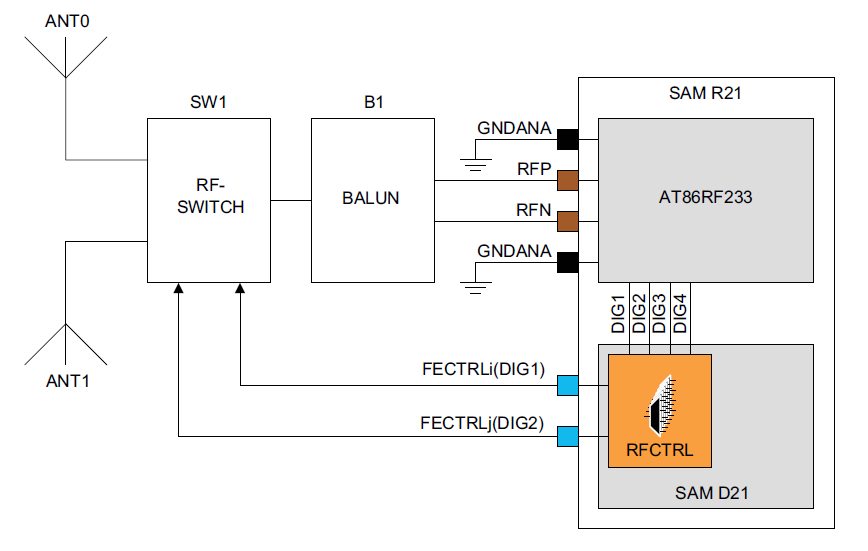
\includegraphics[scale=0.5]{pics/antena.png}
  \caption{Schema de legare a antenei}
  \label{fig:antena}
\end{figure}


\section{Arduino IDE}
Înainte de a trece mai departe, este necesară prezentarea structurii unui proiect din Arduino IDE și detalii despre cum se ajunge la obiectul final încărcat pe placa de dezvoltare țintă.
Un proiect în Arduino IDE este împărțit în 4 părți cu cod sursă:
\begin{itemize}
	\item{core\footnote{core = nucleu} - aici este codul de bază pentru fiecare platformă}
	\item{variant\footnote{variant = se referă la placa de dezvoltare} - aici se află fișiere de configurare pentru placa de dezvoltare}
	\item{sketch\footnote{sketch = schiță} - aici se află codul utilizatorului}
	\item{library\footnote{library = bibliotecă} - aici se află codul sursă pentru bibliotecile opționale}
\end{itemize}
Punctul de intrare în proiect este fișierul \textit{main.c} în funcția \textit{main}, din \textit{core}, în care se apelează funcțiile scrise de utilizator în fișierul cu extensia \textit{.ino}, \textit{setup și loop}, din \textit{sketch}. \\
Procesul de build\footnote{build = construire} al proiecului constă în compilarea tuturor fișierelor sursă, cu fișierele header corespunzătoare, din toate cele 4 părți ale proiectului și asamblarea lor într-un singur fișier rezultat cu extensia \textit{.hex}, stocat la o locație temporară. Fișierul rezultat este mai apoi urcat în memoria microcontrolerului țintă și executat.

\subsection{Dezvoltare proiect}
Pentru a implementa tema propusă, se vor creea 3 din cele 4 părți componente ale unui proietct în Arduino IDE. În final, cele 3 părți formează pachetul care va fi arhivat și stocat online, iar oricine va dori să utilizeze o placă de dezvoltare de acest tip, va putea folosi acest pachet. \\

\subsubsection{Core}
Ținând cont de faptul că placa de dezvoltare Atmel SAM R21 Xplained Pro este un dispozitiv SAM R21,  care este compus din SAM D21 și modulul radio AT86RF233, codul sursă pentru core va fi asemănător cu cel pentru SAM D21, cu modificările aferente pentru configurațiile de pini interni modificați.

\subsubsection{Variant}
În această parte de proiect, este explicată structura și formatul pe care trebuie să-l respecte fișierele componente.

\subsubsection{Library}
Codul sursă pentru funcționalitatea radio se află în această parte a proiectului.

\subsection{Adăugare proiect}
Pentru adăugarea unei noi plăci de dezvoltare la mediul de dezvoltare Arduino IDE, este necesară crearea unui fișier de tip json\footnote{JSON = JavaScript Object Notation} în care se scriu configurațiile pentru pachetul corespunzător plăcii de dezvoltare.
Fișierul json trebuie să conțină următoarele câmpuri:
\begin{itemize}
	\item{name - numele pe care îl va avea pachetul}
	\item{maintainer - numele celui care menține codul}
	\item{websiteURL - un url către un site web al companiei}
	\item{help}
	\item{platforms}
		\subitem{name - numele plăcii de dezvoltare}
		\subitem{arhitecturre - arhitectura pe care se bazează placa de dezvoltare}
		\subitem{version - versiunea pachetului}
		\subitem{category - de obicei este Contributed, doar cei de la Arduino pot schimba}
		\subitem{url - link către o arhivă cu codul sursă}
		\subitem{archiveFilename - numele arhivei}
		\subitem{checksum - pentru verificare se cere un mesaj de autentificare}
		\subitem{size - mărimea arhivei}
		\subitem{boards}
		\subitem{toolsDependencies - secțiunea cu dependențele de alte utilitare}
	\item{tools - aici se specifică explicit de unde se pot luat utilitarele}
\end{itemize}
Un exemplu de fișier de configurare se poate vedea în figura ~\ref{fig:json}.
\begin{figure}[!htb]
\centering
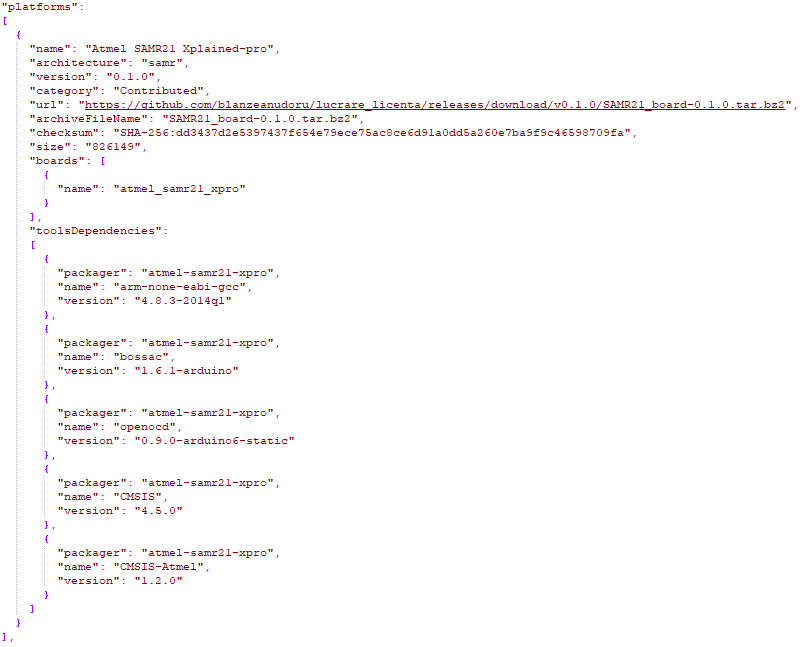
\includegraphics[scale=0.8]{pics/json.png}
  \caption{Exemplu de fișier de configurare}
  \label{fig:json}
\end{figure}


\chapter{Concluzii și dezvoltări ulterioare}


%BIBLIOGRAFIE
\begin{thebibliography}{9}
\bibitem{theiot}
Keyur K Patel, Sunil M Patel. 
\textit{Internet of Things-IOT: Definition, Characteristics, Architecture, Enabling Technologies, Application \& Future Challenges}.
ISSN 2321 3361, 2016 IJESC\\
\href{http://ijesc.org/upload/8e9af2eca2e1119b895544fd60c3b857.Internet\%20of\%20Things-IOT\%20Definition,\%20Characteristics,\%20Architecture,\%20Enabling\%20Technologies,\%20Application\%20\&\%20Future\%20Challenges.pdf}{http://ijesc.org/upload/8e9af2eca2e1119b895544fd60c3b857.Internet\%20of\%20Things-IOT\%20Definition,\%20Characteristics,\%20Architecture,\%20Enabling\%20Technologies,\%20Application\%20\&\%20Future\%20Challenges.pdf}

\bibitem{study}
Padraig Scully.
\textit{The Top 10 IoT Segments in 2018 – based on 1,600 real IoT projects}. 
2018 ranking of Top IoT Segments\\
\href{https://iot-analytics.com/top-10-iot-segments-2018-real-iot-projects/}{https://iot-analytics.com/top-10-iot-segments-2018-real-iot-projects/}

\bibitem{iotfields}
Ran Liu, Jinfeng Wang.
\textit{Internet of Things: Application and Prospect }
MATEC Web of Conferences 100, 02034 (2017)\\
\href{https://www.matec-conferences.org/articles/matecconf/pdf/2017/14/matecconf\_gcmm2017\_02034.pdf}{https://www.matec-conferences.org/articles/matecconf/pdf/2017/14/matecconf\_gcmm2017\_02034.pdf}


\bibitem{lowpowerimportance}
Sayfe Kiaei, Eby G. Friedman.
\textit{Introduction to the Special Issue on Low Power Wireless Communications}.
IEEE TRANSACTIONS ON CIRCUITS AND SYSTEMS—II: ANALOG AND DIGITAL SIGNAL PROCESSING, VOL. 44, NO. 6, JUNE 1997.\\
\href{https://ieeexplore.ieee.org/stamp/stamp.jsp?arnumber=868450}{https://ieeexplore.ieee.org/stamp/stamp.jsp?arnumber=868450}

\bibitem{lowpowervsperformance}
JeongGil Ko, Kevin Klues, Christian Richter, Wanja Hofer, Branislav Kusy, Michael Bruenig, Thomas Schmid, Qiang Wang, Prabal Dutta, and Andreas Terzis
\textit{Low Power or High Performance? A Tradeoff Whose Time Has Come (and Nearly Gone)}\\
\href{https://pdfs.semanticscholar.org/1f68/63c5c7c5e22a4507f1993f6c4c4a8b0b5594.pdf}{https://pdfs.semanticscholar.org/1f68/63c5c7c5e22a4507f1993f6c4c4a8b0b5594.pdf}

\bibitem{samr21ug}
\textit{Atmel-42243D-SAM-R21-Xplained-Pro\_User Guide-04/2016}
\href{http://ww1.microchip.com/downloads/en/DeviceDoc/Atmel-42243-SAMR21-Xplained-Pro-User-Guide.pdf}{http://ww1.microchip.com/downloads/en/DeviceDoc/Atmel-42243-SAMR21-Xplained-Pro-User-Guide.pdf}

\bibitem{antena}
\textit{2.45 GHz SMD Antenna, EIA 1210, Detuning resilient, Edge Mount Design P/N 2450AT18D0100}.
Johanson Technology.
\href{https://www.johansontechnology.com/datasheets/antennas/2450AT18D0100.pdf}{https://www.johansontechnology.com/datasheets/antennas/2450AT18D0100.pdf}

\bibitem{at86rf}
AT86RF233. 
\textit{Low Power, 2.4GHz Transceiver for ZigBee, RF4CE, IEEE 802.15.4, 6LoWPAN, and ISM Applications}.
\href{http://ww1.microchip.com/downloads/en/DeviceDoc/atmel-8351-mcu\_wireless-at86rf233\_datasheet.pdf}{http://ww1.microchip.com/downloads/en/DeviceDoc/atmel-8351-mcu\_wireless-at86rf233\_datasheet.pdf}

\bibitem{switch}
\textit{AS222-92, AS222-92LF: PHEMT GaAs IC SPDT Switch 0.1–3 GHz}.
\href{http://www.skyworksinc.com/uploads/documents/200252C.pdf}{http://www.skyworksinc.com/uploads/documents/200252C.pdf}

\bibitem{balun}
\textit{2.45GHz Impedance Matched Balun-Filter for Atmel Chipset AT86RF232 and AT86RF233}.
\href{https://www.johansontechnology.com/datasheets/balun-filter/2450BM15A0015.pdf}{https://www.johansontechnology.com/datasheets/balun-filter/2450BM15A0015.pdf}

\bibitem{cpu}
\textit{Cortex-M0+ Devices}.
Generic User Guide.
\href{http://infocenter.arm.com/help/topic/com.arm.doc.dui0662b/DUI0662B\_cortex\_m0p\_r0p1\_dgug.pdf}{http://infocenter.arm.com/help/topic/com.arm.doc.dui0662b/DUI0662B\_cortex\_m0p\_r0p1\_dgug.pdf}


\end{thebibliography}

\end{document}